\documentclass[tikz,border=6pt]{standalone}
\usepackage{fontspec}
\setmainfont{Noto Sans}
\usepackage{amsmath}
\usepackage{tikz}
\usetikzlibrary{arrows.meta,positioning}
\definecolor{cudaG}{RGB}{118,185,0}
\definecolor{gsBlue}{RGB}{40,110,190}
\definecolor{pyYel}{RGB}{240,170,30}
\definecolor{secG}{RGB}{85,85,85}
\begin{document}
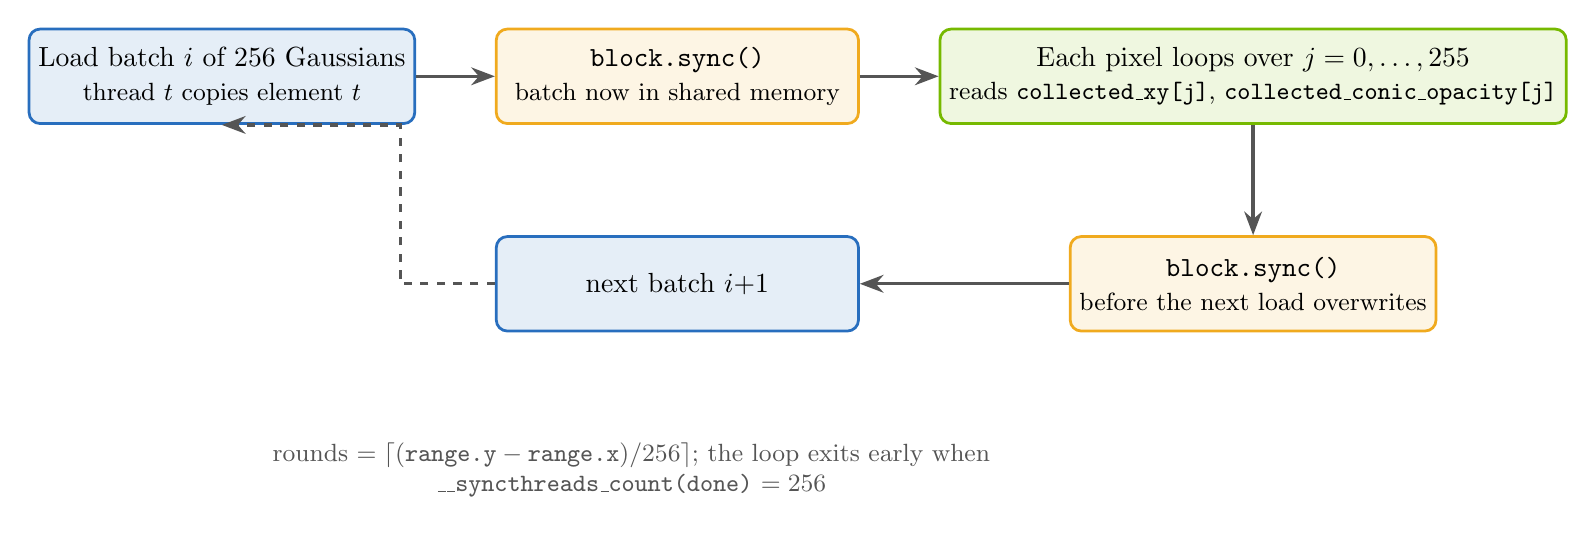
\begin{tikzpicture}[font=\sffamily]
  \tikzset{st/.style={draw=#1,line width=1pt,rounded corners,fill=#1!12,minimum width=4.6cm,minimum height=1.2cm,align=center,font=\normalsize}}
  \node[st=gsBlue] (a) at (0,0) {Load batch $i$ of 256 Gaussians\\{\small thread $t$ copies element $t$}};
  \node[st=pyYel,right=1.0cm of a] (b) {\texttt{block.sync()}\\{\small batch now in shared memory}};
  \node[st=cudaG,right=1.0cm of b] (c) {Each pixel loops over $j=0,\dots,255$\\{\small reads \texttt{collected\_xy[j]}, \texttt{collected\_conic\_opacity[j]}}};
  \node[st=pyYel,below=1.4cm of c] (d) {\texttt{block.sync()}\\{\small before the next load overwrites}};
  \node[st=gsBlue,below=1.4cm of b] (e) {next batch $i{+}1$};
  \draw[-{Stealth[length=3mm]},line width=1.2pt,secG] (a) -- (b);
  \draw[-{Stealth[length=3mm]},line width=1.2pt,secG] (b) -- (c);
  \draw[-{Stealth[length=3mm]},line width=1.2pt,secG] (c) -- (d);
  \draw[-{Stealth[length=3mm]},line width=1.2pt,secG] (d) -- (e);
  \draw[-{Stealth[length=3mm]},line width=1.2pt,secG,dashed] (e.west) -- ++(-1.2,0) |- (a.south);
  \node[font=\small,secG,align=center] at (5.2,-5.0) {rounds $=\lceil(\texttt{range.y}-\texttt{range.x})/256\rceil$; the loop exits early when\\\texttt{\_\_syncthreads\_count(done)} $=256$};
\end{tikzpicture}
\end{document}
